\chapter{Version Space Algebra}
\label{ch:vsa}

A typical practical DSL may have up to $10^{30}$ programs consistent with a given spec~\cite{vldb12:semantic}.
Solving a synthesis problem over such a DSL requires a data structure for succinctly representing such a huge number of
programs in polynomial space.
Such a data structure, called \emph{version space algebra} (VSA),
was defined by Mitchell~\cite{vsa:Mitchell} in the context of machine learning, and later used for programming by demonstration in
SMARTedit~\cite{lau:smartedit}, FlashFill~\cite{flashfill}, and other synthesis applications.
Its efficiency is based on the fact that typically many of these $10^{30}$ programs share common subexpressions.
In this section, I formalize the generic definition of VSA as an essential primitive for synthesis algorithms, expanding
upon specific applications that were explored previously by \citeauthor{vsa:Mitchell}, \citeauthor{lau:smartedit},
\citeauthor{flashfill}, and others.
I define a set of efficient operations over this data structure that are used by several synthesis algorithms,
including the deductive algorithm of \PROSE.

Intuitively, a VSA can be viewed as a directed graph where each node represents a set of programs.
A leaf node in this graph is annotated with a \emph{direct} set of programs, and it explicitly represents this set.
There are also two kinds of internal (constructor) nodes.
A \emph{union} VSA node represents a set-theoretic union of the program sets represented by its children VSAs.
A \emph{join} VSA node with $k$ children VSAs is annotated with a $k$-ary DSL operator $F$, and it represents a cross
product of all possible applications of $F$ to $k$ parameter programs, independently chosen from the children VSAs.
Hereinafter I use the words ``program set'' and ``version space algebra'' interchangeably, and use the same notation for both concepts.

\begin{defn}[Version space algebra]
    \label{def:vsa}
    Let $\dsl$ be a DSL.
    A \emph{version space algebra} is a representation for a set $\vsa$ of programs rooted at the same symbol of $\dsl$,
    with the following grammar:
    \begin{align*}
        \vsa \is \left\{P_1, \dots, P_k\right\} \,\palt\, \vsaunion(\vsa_1, \dots, \vsa_k) \,\palt\, \joinCons(\vsa_1, \dots, \vsa_k)
    \end{align*}
    where $F$ is any $k$-ary operator in $\dsl$.
    The semantics of VSA as a set of programs is as follows:
    \begin{align*}
        &P \in \left\{P_1, \dots P_k\right\} \tag*{if $\exists\, j\colon P = P_j$} \\
        &P \in \vsaunion(\vsa_1, \dots, \vsa_k) \tag*{if $\exists\, j\colon P \in \vsa_j$} \\
        &P \in \joinCons(\vsa_1, \dotsc, \vsa_k) \tag*{if $P = F(P_1, \dots, P_k) \ \wedge\ \forall j\colon P_j \in \vsa_j$}
    \end{align*}
\end{defn}

\begin{defn}[VSA size, width, and volume]
    Given a VSA $\vsa$, the \emph{size} of $\vsa$, denoted $|\vsa|$, is the number of programs in the set
    represented by $\vsa$, the \emph{width} of $\vsa$, denoted $\width{\vsa}$, is the maximum number of children
    in any constructor node of $\vsa$, and the \emph{volume} of $\vsa$, denoted $\volume{\vsa}$, is the number of nodes in $\vsa$.
\end{defn}

Note that programs in a VSA can benefit from two kinds of sharing of common subexpressions.
One sharing happens via join VSA nodes, which succinctly represent a cross product of possible subexpression
combinations.
Another sharing happens by virtue of having multiple incoming edges into a VSA node (i.e. two identical program sets are
represented with one VSA instance in memory).
Therefore in common (non-degenerate) cases $\volume{\vsa} = \mathcal{O}(\log |\vsa|)$.

\begin{example}
    \Cref{fig:ex:vsa} shows a VSA of all FlashFill programs that output the string \stringliteral{425} on a given input state
    $\state = \left\{ v_1 \mapsto \stringliteral{(425) 555-7709}\right\}$.
    The string \stringliteral{425} can be represented in four possible ways as a concatenation of individual substrings.
    Each substring of \stringliteral{425} can be produced by a \textsf{ConstStr} program or a \textsf{SubStr} program.
\end{example}

\begin{figure}[t]
    \centering
    % \uwsinglespace
    \begin{dot2tex}[options=--usepdflatex --figonly]
        
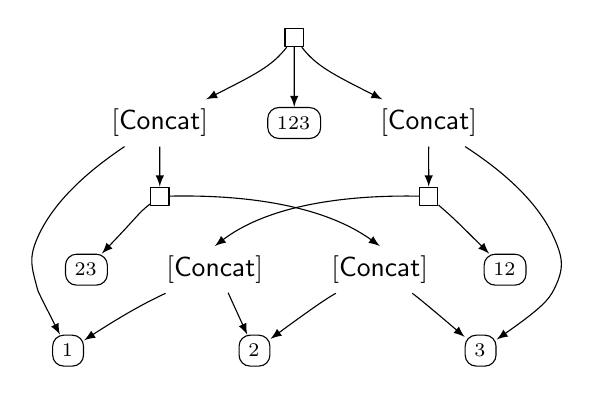
\begin{tikzpicture}[>=latex,line join=bevel,scale=1.1]
%%
\begin{scope}
  \pgfsetstrokecolor{black}
  \definecolor{strokecol}{rgb}{1.0,1.0,1.0};
  \pgfsetstrokecolor{strokecol}
  \definecolor{fillcol}{rgb}{1.0,1.0,1.0};
  \pgfsetfillcolor{fillcol}
\end{scope}
  \node (concat1o23) at (41.999bp,81.5bp)  {$\joinCons[\mathsf{Concat}]$};
  \node (const23) at (17.999bp,33.5bp) [draw,rectangle,rounded corners] {$\vsa_{23}$};
  \node (e23) at (41.999bp,57.5bp) [draw,rectangle] {$\vsaunion$};
  \node (e12) at (130.0bp,57.5bp) [draw,rectangle] {$\vsaunion$};
  \node (e123) at (85.999bp,109.5bp) [draw,rectangle] {$\vsaunion$};
  \node (concat12) at (59.999bp,33.5bp)  {$\joinCons[\mathsf{Concat}]$};
  \node (const12) at (155.0bp,33.5bp) [draw,rectangle,rounded corners] {$\vsa_{12}$};
  \node (concat12o3) at (130.0bp,81.5bp)  {$\joinCons[\mathsf{Concat}]$};
  \node (const123) at (85.999bp,81.5bp) [draw,rectangle,rounded corners] {$\vsa_{123}$};
  \node (e2) at (72.999bp,7.0bp) [draw,rectangle,rounded corners] {$\vsa_2$};
  \node (e1) at (11.999bp,7.0bp) [draw,rectangle,rounded corners] {$\vsa_1$};
  \node (e3) at (147.0bp,7.0bp) [draw,rectangle,rounded corners] {$\vsa_3$};
  \node (concat23) at (114.0bp,33.5bp)  {$\joinCons[\mathsf{Concat}]$};
  \draw [->] (concat12o3) ..controls (153.11bp,66.505bp) and (165.38bp,56.521bp)  .. (171.0bp,44.0bp) .. controls (174.09bp,37.106bp) and (174.38bp,33.758bp)  .. (171.0bp,27.0bp) .. controls (169.32bp,23.637bp) and (166.68bp,20.74bp)  .. (e3);
  \draw [->] (e12) ..controls (114.99bp,57.75bp) and (81.517bp,57.677bp)  .. (concat12.north);
  \draw [->] (e123.south) ..controls (85.999bp,100.65bp) and (85.999bp,100.3bp)  .. (const123);
  \draw [->] (concat12) ..controls (40.603bp,24.196bp) and (33.585bp,20.999bp)  .. (e1);
  \draw [->] (e23) ..controls (57.222bp,57.793bp) and (91.174bp,57.809bp)  .. (concat23.north);
  \draw [->,draw=none] (concat1o23) ..controls (63.422bp,81.5bp) and (63.533bp,81.5bp)  .. (const123);
  \draw [->] (e123) ..controls (93.296bp,100.02bp) and (98.949bp,97.319bp)  .. (concat12o3);
  \draw [->] (e12) ..controls (136.63bp,51.611bp) and (136.67bp,51.9bp)  .. (const12);
  \draw [->] (e23) ..controls (34.654bp,51.698bp) and (35.858bp,52.127bp)  .. (const23);
  \draw [->] (concat23) ..controls (125.45bp,25.165bp) and (128.1bp,23.171bp)  .. (e3);
  \draw [->,draw=none] (const123) ..controls (98.139bp,81.5bp) and (98.249bp,81.5bp)  .. (concat12o3);
  \draw [->] (concat1o23) ..controls (19.437bp,66.386bp) and (7.464bp,56.385bp)  .. (1.9989bp,44.0bp) .. controls (-1.0513bp,37.087bp) and (0.10366bp,34.314bp)  .. (1.9989bp,27.0bp) .. controls (2.12bp,26.533bp) and (2.2561bp,26.065bp)  .. (e1);
  \draw [->] (concat12o3) ..controls (130.0bp,72.684bp) and (130.0bp,72.446bp)  .. (e12);
  \draw [->] (e123) ..controls (78.702bp,100.02bp) and (73.049bp,97.319bp)  .. (concat1o23);
  \draw [->] (concat1o23) ..controls (41.999bp,72.684bp) and (41.999bp,72.446bp)  .. (e23);
  \draw [->] (concat23) ..controls (97.584bp,24.673bp) and (93.518bp,22.081bp)  .. (e2);
  \draw [->] (concat12) ..controls (64.101bp,26.455bp) and (64.38bp,25.907bp)  .. (e2);
%
\end{tikzpicture}


    \end{dot2tex}
    \caption{A VSA representing all possible programs output the string \stringliteral{425} in $\ffdsl$.
    Leaf nodes $\vsa_1, \vsa_2, \vsa_3, \vsa_{12}, \vsa_{23}$ are VSAs representing all ways to output substrings
    \stringliteral{4}, \stringliteral{2}, \stringliteral{5}, \stringliteral{42}, and \stringliteral{25} respectively
    (not expanded in the figure).}
    \label{fig:ex:vsa}
\end{figure}

I define three operations over VSAs, which are used during the synthesis process: \emph{intersection},
\emph{ranking}, and \emph{clustering}.
Intersection of VSAs was first used by Lau et al.~\cite{lau:smartedit} and then adapted by us for FlashFill~\cite{flashfill}.
It has been defined specifically for VSAs built on the SMARTedit and FlashFill DSLs.
In this section, I define VSA intersection generically, and also introduce ranking and clustering of VSAs, which are
novel contributions of this thesis.

\section{Intersection}
Intersection of VSAs enables quick unification of two sets of candidate programs that are consistent with two different
specs.
Given a conjunctive spec $\spec_1 \wedge \spec_2$, one possible synthesis approach is to learn a set of programs
$\vsa_1$ consistent with
$\spec_1$, another set of programs $\vsa_2$ consistent with $\spec_2$, and then intersect $\vsa_1$ with $\vsa_2$.
An efficient algorithm for VSA intersection follows the ideas of automata intersection \cite{hopcroft1979introduction}.

\begin{defn}[Intersection of VSAs]
    \label{def:intersection}
    Given VSAs $\vsa_1$ and $\vsa_2$, their \emph{intersection} $\vsa_1 \cap \vsa_2$ is a VSA that
    contains those and only those programs that belong to both $\vsa_1$ and $\vsa_2$.
    Constructively, it is defined as follows (modulo symmetry):
    \begingroup\allowdisplaybreaks
    \begin{align*}
        \bigl[\vsaunion(\vsa'_1, \dots, \vsa'_k)\bigr] \cap \vsa_2 &\bydef \vsaunion\,(\vsa'_1 \cap \vsa_2,
            \dots, \vsa'_k \cap \vsa_2) \\
        \joinCons(\vsa'_1, \dots, \vsa'_k) \cap \joinCons[G](\vsa''_1, \dots, \vsa''_m) &\bydef \emptyset \\
        \joinCons(\vsa'_1, \dots, \vsa'_k) \cap \joinCons(\vsa''_1, \dots, \vsa''_k) &\bydef
        \joinCons(\vsa'_1 \cap \vsa''_1, \dots, \vsa'_k \cap \vsa''_k) \\
        \joinCons(\vsa'_1, \dots, \vsa'_k) \cap \left\{P_1, \dots, P_m\right\} &\bydef
        \bigl\{P_j = F(P'_1, \dots, P'_k) \mid P'_j \in \vsa'_j\bigr\} \\
        \vsa_1 \cap \vsa_2 &\bydef \vsa_1 \cap \vsa_2\ \text{ as direct program sets otherwise}
    \end{align*}%
    \endgroup
\end{defn}

\begin{theorem}
    $\volume{\vsa_1 \cap \vsa_2} = \mathcal{O}(\volume{\vsa_1} \cdot \volume{\vsa_2})$.
\end{theorem}
\begin{proof}
    Follows by induction over the structure of $\vsa_1$ and $\vsa_2$ in~\Cref{def:intersection}.
    The only non-trivial case is union intersection $[ \vsaunion(\vsa'_1, \dots, \vsa'_k)] \cap [ \vsaunion(\vsa''_1,
    \dots, \vsa''_m) ]$, which introduces $k \cdot m$ constructors per level in $\vsa_1 \cap \vsa_2$.
\end{proof}

\section{Ranking}
Ranking of VSAs enables us to quickly select the topmost-ranked programs in a set of ambiguous candidates with respect
to some domain-specific ranking function.

\begin{defn}[Ranking of a VSA]
    Given a VSA $\vsa$, a ranking function $\rank\colon\dsl\to\Reals$, and an integer $k \ge 1$, the operation
    $\mathsf{Top}_{\rank}(\vsa, k)$ returns a (sorted) set of programs that correspond to $k$ highest values of $\rank$ in $\vsa$.
    % For example:
    % \begin{align*}
    %     \mathsf{Top}_{\rank}(\vsa, 1) = \Argmax\nolimits_{P \in \vsa} \rank(P)
    % \end{align*}
\end{defn}

$\mathsf{Top}_{\rank}(\vsa, k)$ can be defined constructively, provided the ranking function $h$ is \emph{monotonic} over the
program structure (i.e. provided $h(P_1) > h(P_2) \,\Rightarrow\, h(F(P_1)) > h(F(P_2))$):
\begin{align*}
    \mathsf{Top}_{\rank}(\left\{P_1,\dots,P_m\right\}, k) &\bydef \mathsf{Select}(\rank, k, \left\{P_1,\dots,P_m\right\}) \\
    \mathsf{Top}_{\rank}(\vsaunion(\vsa_1,\dots,\vsa_m), k) &\bydef \mathsf{Select}\bigl(\rank, k, \cup_{i=1}^n
    \mathsf{Top}_{\rank}(\vsa_i, k)\bigr) \\
    \mathsf{Top}_{\rank}(\joinCons(\vsa_1,\dots,\vsa_m), k) &\bydef
    \mathsf{Select}\bigl(\rank, k, \bigl\{F(P_1,\dots, P_m) \mid \forall i\ P_i \in \mathsf{Top}_{\rank}(\vsa_i, k)\bigr\} \bigr)
\end{align*}
\noindent Here $\mathsf{Select}$ function implements a \emph{selection algorithm} for top $k$ elements among $\left\{P_1, \dots, P_m\right\}$
according to the ranking function $\rank$.
It can be efficiently implemented either in $\mathcal{O}(m + k \log k)$ time
using Hoare's \texttt{quickselect} algorithm~\cite{quickselect}, or in $\mathcal{O}(m \log k)$ time using a heap.

\begin{theorem}
    \label{thm:vsa:ranking}
    Let $\vsa$ be a VSA, and let $m = \width{\vsa}$.
    Assume $\mathcal{O}(m \log k)$ implementation of the $\mathsf{Select}$ function.
    The time complexity of calculating $\mathsf{Top}(\vsa, k)$ is $\mathcal{O}(\volume{\vsa}\, k^m \log k)$.
\end{theorem}
\begin{proof}
    Let $d$ be the depth (number of levels) of $\vsa$.
    Note that $\volume{\vsa} = \mathcal{O}(m^d)$.
    Let $T(n)$ denote the time complexity of calculating $\mathsf{Top}_{\rank}(\vsa_{(n)}, k)$, where $\vsa_{(n)}$ is the
    $n^{\text{th}}$ level of $\vsa$.
    For a leaf node we have $T(1) = \mathcal{O}(m \log k)$.
    For a union node we have $T(n) = \mathcal{O}(m \cdot T(n-1) + k\, m \log k)$, where the first term represents calculation of
    $\mathsf{Top}_{\rank}$ over the children, and the second term represents the selection algorithm.
    For a join node we similarly have $T(n) = \mathcal{O}(m\cdot T(n-1) + k^m \log k)$.
    Since $T(n)$ grows faster if $\vsa_{(n)}$ is a join rather than a union, we can ignore the non-dominant union case.
    Solving the recurrence for $T(n)$, we get:
    \addtolength{\jot}{-1pt}
    \begin{align*}
        T(d) &=\ \mathcal{O}\left( m^d \log k + (m-1)^{-1} k^m (m^{d-1}-1) \log k \right)
        = \mathcal{O}(m^d k^m \log k) = \mathcal{O}(\volume{\vsa} \cdot k^m \log k) \ \ \qedhere
    \end{align*}
\end{proof}

\section{Clustering}
Clustering of a VSA partitions it into subsets of programs that are semantically indistinguishable w.r.t. the given
input state $\state$, i.e. they give the same output on $\state$.
This operation enables efficient implementation of various computations over a set of candidate programs (e.g.,
filtering or splitting into independent search subspaces).

\begin{defn}[Clustering of a VSA]
    Given a VSA $\vsa$ and an input state $\state$ over $\freeVariables{N}$, the \emph{clustering} of
    $\vsa$ on~$\state$, denoted $\clustering$, is a mapping
    $\{ v_1\mapsto \vsa_1,\dots,v_n\mapsto \vsa_n\}$ such that:
    \begin{enumerate}[label=\textbf{(\alph*)},nosep]
        \item $\vsa_1 \cup \dots \cup \vsa_n = \vsa$.
        \item $\vsa_i \cap \vsa_j = \emptyset$ for all $i \ne j$.
        \item For any $P \in \vsa_j\colon\ \semantics{P}{\state} = v_j$.
        \item For any $i \ne j\colon\ v_i \ne v_j$.
    \end{enumerate}
    \noindent In other words, $\clustering$ is a partitioning of $\vsa$ into non\hyp{}intersecting subsets of programs, where
    each subset contains the programs that give the same output $v$ on the given input state~$\state$.
    We can also straightforwardly lift the clustering operation onto tuples of input states $\states$, partitioning $\vsa$ into subsets of
    programs that given the same output $\values$ on $\states$.
\end{defn}

Constructively, $\clustering$ is defined as follows:
\begin{align*}
    \clustering[\left\{P_1, \dots, P_k\right\}] &\bydef \mathsf{G}\bigl( \{ \semantics{P_i}{\state} \mapsto \{P_i\} \bigmid i = 1..k \} \bigr) & \\
    \clustering[\vsaunion(\vsa_1,\dots,\vsa_k)] &\bydef \mathsf{G}\bigl(\textstyle\bigvsaunion\nolimits_k
        \clustering[\vsa_k]\bigr) & \\
    \clustering[\joinCons(\vsa_1,\dots,\vsa_k)] &\bydef
        \mathsf{G}\bigl( \bigl\{ \semantics{F(v_1,\dots,v_k)}{\state} \mapsto \joinCons(\vsa'_1,\dots,\vsa'_k)
        \bigmid \langle v_j, \vsa'_j \rangle\in \clustering[\vsa_j][\state_j] \bigr\} \bigr)
\end{align*}
where $\state_1,\dots,\state_k$ are input states passed by $F$ into its arguments during execution on $\state$, and
\begin{align*}
    &\mathsf{G}(\{ v_1\mapsto \vsa_1,\dots,v_n\mapsto \vsa_n \}) \bydef
    \bigl\{ v \mapsto \bigvsaunion\limits_{v \mapsto \vsa_j} \vsa_j \bigmid \text{all unique } v \text{ among } v_j \bigr\}
\end{align*}
is a ``group-by'' function.
It groups a given set of bindings by keys, uniting VSAs that correspond to the same key with a $\vsaunion$
constructor.

The clustering operation allows us to answer many questions about the current set of candidate programs efficiently.
For example, it allows us to efficiently filter out the programs in $\vsa$ that are inconsistent with a given spec:
\begin{defn}[Filtered VSA]
    Given a VSA $\vsa$ and a spec $\spec$ on $N$, a \emph{filtered VSA} $\mathsf{Filter}(\vsa, \spec)$ is defined as
    follows: $\mathsf{Filter}(\vsa, \spec) \bydef \bigl\{P \in \vsa \mid P \models \spec\bigr\}$.
    \label{def:vsa:filtered}
\end{defn}
\begin{theorem}
    If $\states$ is a state tuple associated with $\spec$, then:
    \begin{enumerate}[nosep,label=(\arabic*)]
        \item $\mathsf{Filter}(\vsa, \spec) = \bigvsaunion\bigl\{\vsa_j \bigmid \langle \values_j \mapsto \vsa_j \rangle
                \in \clustering[\vsa][\states] \ \wedge\  \spec(\values_j)\bigr\}$.
        \item The construction of $\mathsf{Filter}(\vsa, \spec)$ according to (1) takes
            $\mathcal{O}\bigl(\bigl|\clustering[\vsa][\states]\bigr|\bigr)$ time after the clustering.
    \end{enumerate}
\end{theorem}
\begin{proof}
    Follows by construction from \Cref{def:vsa:filtered}.
\end{proof}

Estimating the size of $\clustering[\vsa][\states]$ and the running time of clustering is difficult, since these values
depend not only on $\vsa$ and $\state$, but also on the semantics of the operators in $\dsl$ and the number of
collisions in their possible output values.
However, in \Cref{sec:experiments} I show that these values usually remain small for any practical DSL.

\section{VSA as a Language}
\label{sec:vsa:language}

\begin{figure}[t]
    \uwsinglespace
    \begin{minipage}[b]{0.42\textwidth}
        \begin{lstlisting}[language=dsl, gobble=12]
            int $position$[string $s$] $\coloneqq$
                AbsPos($s$, $k$)
              | RegexPos($s$, std.Pair($r$, $r$), $k$);
            int $k$;
            Regex $r$;
        \end{lstlisting}
    \end{minipage}
    \hspace*{-5pt}
    \begin{minipage}[t]{0.577\textwidth}
        \small
        \begin{dot2tex}[options=--usepdflatex --figonly]
            \input{vsa/language-repr.dot}
        \end{dot2tex}
    \end{minipage}
    \vspace*{-\baselineskip}
    \caption{
        A VSA can be seen as an isomorphic representation for a CFG of some sub-language of the original DSL.
        \emph{Left:} An excerpt from the FlashFill DSL definition.
        \emph{Right:} A sample VSA that represents a sub-language of the DSL on the top.}
    \label{fig:vsa:language-repr}
\end{figure}

\begin{figure}[t]
    \centering
    % \uwsinglespace
    \small
    \begin{algorithmic}[1]
        \Functionx{VsaToDsl}{VSA $\vsa$}
            \State Let $V$ be a set of fresh nonterminals, one per each non-leaf node in $\vsa$
            \State Let $\Sigma$ be a set of fresh terminals, one per each leaf node in $\vsa$
            \State \Comment{We write $\mathsf{sym}(\vsa') \in V \cup \Sigma$ to denote the corresponding fresh symbol
                for a node $\vsa'$ from $\vsa$}
            \addtocounter{ALG@line}{-1}
            \WithNumber \State Productions $R \gets \emptyset$
            \State \Comment{Create ``symbol $:=$ symbol'' productions for all union nodes}
            \ForAll{union nodes $\vsa' = \vsaunion(\vsa_1, \dots, \vsa_k)$ in $\vsa$}
                \State $R \gets R \cup \{ \mathsf{sym}(\vsa') := \mathsf{sym}(\vsa_i) \mid i = 1 \dots k \}$
            \EndFor
            \State \Comment{Create operator productions for all join nodes}
            \ForAll{join nodes $\vsa' = \vsajoin(\vsa_1, \dots, \vsa_k)$ in $\vsa$}
                \State $R \gets R \cup \{ \mathsf{sym}(\vsa') := F(\mathsf{sym}(\vsa_1), \dots, \mathsf{sym}(\vsa_k)) \}$
            \EndFor
            \State \Comment{Annotate terminal symbols with values extracted from leaf nodes}
            \ForAll{leaf nodes $\vsa' = \{ P_1, \dots, P_k \}$ in $\vsa$}
                \State Annotate in $\Sigma$ that $\mathsf{sym}(\vsa') \in \{ P_1, \dots, P_k \}$
            \EndFor
            \State \Return the context-free grammar $G = \langle V, \Sigma, R, \mathsf{sym}(\vsa)\rangle$
        \EndFunction
    \end{algorithmic}
    \caption{An algorithm for translating a VSA $\vsa$ of programs in a DSL $\dsl$ into an isomorphic grammar for a
        sub-DSL $\dsl' \subset \dsl$.}
    \label{fig:vsa:incremental}
\end{figure}

Another view on a version space algebra is that it is a different representation of a \emph{language}, isomorphic to a
context-free grammar (CFG).
In formal logic, a language is defined as a set of programs.
We commonly represent languages as CFGs, which are based on two syntactic features: \emph{union of rules} ($|$) and
\emph{sharing of nonterminals}.
A VSA is also a representation for a set of programs; it is an AST-based representation that leverages
two syntactic features: \emph{union} ($\vsaunion$) and \emph{join of shared VSAs} ($\joinCons$).
These representations are isomorphic; in fact, a VSA built from a DSL $\dsl$ is essentially a CFG for some DSL $\dsl'
\subseteq \dsl$.
For instance, \Cref{fig:vsa:language-repr} shows an example of a small DSL (an excerpt from FlashFill) and a VSA that
represents a finite sub-language of this DSL.

This observation is important because it allows us (with careful implementation) to treat VSAs and CFGs interchangeably.
Such treatment is the main driver behind seamless \emph{incremental program synthesis} in the PROSE framework, which I
describe in \Cref{sec:interactive:incremental}.

\Cref{fig:vsa:incremental} shows an algorithm for translating $\vsa$ into a grammar of $\dsl'$.
It performs an isomorphic graph translation, converting VSA unions ($\vsaunion$) into CFG alternatives ($N := N_1 \palt
N_2$), VSA joins~($\vsajoin$) into CFG operator productions ($N := F(\dots)$), and explicit program sets into CFG
terminals annotated with their possible values.
